%=============================
%=============================
% \subsection{Modèles et standards de description}
\subsection{Dublin Core Metadata Initiative: Metadata Terms}
\begin{table}[htb!]
   \begin{center}
		\begin{tabularx}{0.75\textwidth}{l X}
		   \hline
\gpc{Propriété} & \gpc{Sous-propriétés} \\ \hline
accrualMethod & \\ \hline
accrualPeriodicity & \\ \hline
accrualPolicy & \\ \hline
audience & 
	educationLevel, mediator\\ \hline
\e{contributor} & 
	\e{creator} \\ \hline
\e{coverage} & 
	spatial, temporal \\ \hline
\e{date} & 
	available, created, dateAccepted, dateCopyrighted, dateSubmitted, issued, modified,	valid  \\ \hline

\e{description} & 
	abstract, tableOfContents \\ \hline
\e{format} & 
	extent, medium \\ \hline
\e{identifier} & 
	bibliographicCitation \\ \hline

instructionalMethod & \\ \hline
\e{language} & \\ \hline
provenance & \\ \hline
\e{publisher} & \\ \hline
\e{relation} &
	conformsTo, hasFormat, hasPart, hasVersion, isFormatOf,	isPartOf, 	isReferencedBy, isReplacedBy, isRequiredBy, isVersionOf, references, replaces, requires, \e{source} \\ \hline 
\e{rights} & 
	accessRights, license \\ \hline
rightsHolder & \\ \hline
\e{subject} & \\ \hline
\e{title} & 
	alternative \\ \hline
\e{type} & \\ \hline
		\end{tabularx}
		\caption{Liste des propriétés et sous-propriétés du DCMI Metadata Terms \label{tab:dcmi}}
   \end{center}
\end{table}

La \pc{Dublin Core Metadata Initiative} (DCMI) est une organisation qui vise à développer et promouvoir l'usage de standards de description de ressources afin de faciliter l'échange d'information sur le Web.
Depuis la première conférence organisé en 1995 à Dublin, Ohio, l'organisation a enrichi le vocabulaire de son standard original, le \pc{Dublic Core Metadata Element Set} (DCMES), de nouveaux éléments. 
En effet, la version étendue de \pc{DCMI Metadata Terms} (\cite{DCMIUsageBoard2010}) compte 54 propriétés et sous-propriétés, dont les 15 éléments d'origines (marqués en \e{italique} dans la Table \ref{tab:dcmi}).
L'intérêt de cette structuration est de pouvoir remplacer les valeurs des sous-propriétés comme des valeurs de leur propriété parente. 
La structuration des propriétés est telle que la valeur conserve une signification, même si celle-ci correspond à une propriété est moins précise. 
Cela sert notamment pour réaliser des inférences et de l'enrichissement de requêtes.

\begin{figure}[ht!]
\centering
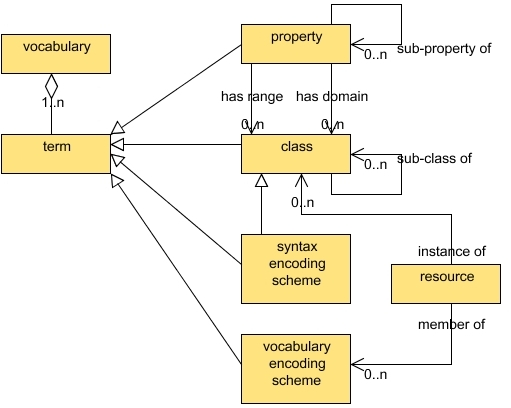
\includegraphics[width=0.6\textwidth]{images/vocabulary-model.jpg}
\caption{Modèle général du DCMI}
\label{img:dcmi-voc}
\end{figure}

\paragraph{Modèle général et représentation}
Une des grandes avancées de \cite{DCMIUsageBoard2010}, a été la constitution d'une modélisation générale, voir la Figure \ref{img:dcmi-voc}, et l'introduction d'une syntaxe de représentation utilisants XML, RDF et RDF-S. 
En plus des propriétés, le modèle définit la notion de Classe et de Schéma d'encodage (qui sera expliqué ci-après). 
Les classes permettent de définir des types de ressources et de leur attribuer des URI. 

Chaque \pc{Terme} est défini par une liste d'attributs lui donnant un identifiant, une étiquette, une définition, ajoutant des commentaires, de la documentation, une référence complémentaire, les relations hiérarchiques avec les autres Termes, la classe et le type du Terme, l'appartenance à un Schéma d'encodage, les restrictions de sujet et d'objet qui s'applique à une propriété, les propriétés équivalentes.
Ainsi, on peut maintenant utiliser des URI, faisant référence à d'autres ressources, comme valeur d'une propriété.
Les valeurs peuvent donc être soit une expression littérale, une URI quelconque, ou bien une URI pointant vers un type de ressource particulier, comme un Terme appartenant à un schéma d'encodage ou une classe.
Par exemple, la propriété \pc{creator} ne peut pointer que vers des ressources de classe \pc{Agent} (du fait d'une restriction \pc{hasRange}). 


\paragraph{Schémas d'encodage}
Il existe deux types de schémas d'encodage qui permettent de préciser si les valeurs des propriétés sont écrites selon une syntaxe particulière (\pc{Syntax Encoding Scheme}, SES), ou si la valeur fait partie d'un thésaurus ou d'un vocabulaire contrôlé (\pc{Vocabulary Encoding Scheme}, VES).
Cela permet par exemple, d'indiquer que les valeurs de la propriété \pc{date} sont écrites suivant le format du W3C Date Time Format ou bien suivant la norme ISO 8106. 
De même, on peut déclarer que les valeurs de la propriété \pc{subject} seront prises dans la liste des \pc{Library of Congress Subject Headings}. 
%need REF ! 
SES et VES offrent ainsi la possibilité d'utiliser plusieurs jargons ou syntaxes pour caractériser les valeurs des propriétés, voir [A1] dans les besoins de modélisations du chapitre précédent (\ref{sec:bm}).
De plus, la spécification d'un Terme permet d'ajouter une définition et de pointer vers d'autres ressources pour documenter les Termes, voir [A2].

\begin{figure}[ht!]
\centering
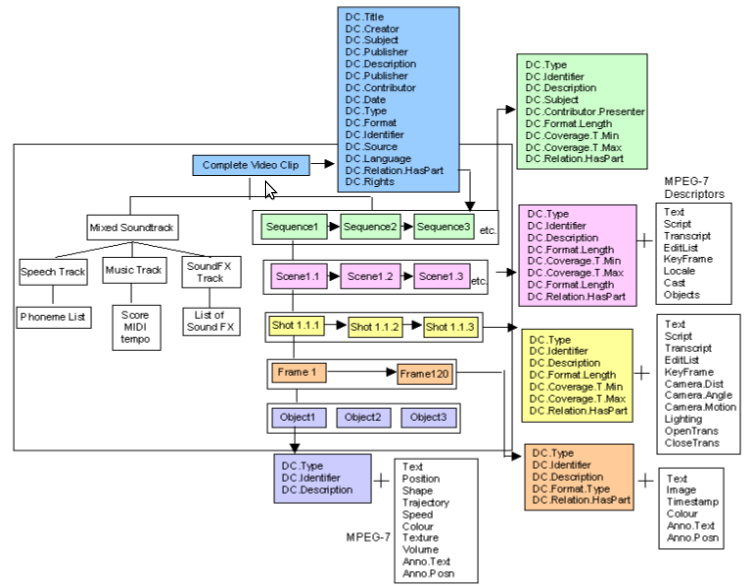
\includegraphics[width=0.8\textwidth]{images/HunterDCMI-MPEG7.png}
\caption{Modèle de Dublin Core étendu pour l'audiovisuel avec des descripteurs MPEG-7 (\cite{Hunter1999})}
\label{img:dcmi-mpeg7}
\end{figure}


\paragraph{Application à l'audiovisuel}
La modélisation du DCMI Metadata Terms s'intéresse à la description de tout types de ressources sur le Web (ce qui est identifié par une URI \cite{Berners-Lee1998}).
Cette perspective très générique lui permet de s'appliquer à de nombreux cas d'usages sans pour autant traiter leurs spécificités. 
Ainsi, dans le cas de l'audiovisuel il faudrait étendre ce schéma pour décrire par exemple le format d'image, les différents contributeurs, inclure de nouveaux types de dates, de nouvelles classes de Termes etc.

\cite{Hunter1998} ont proposés une extension qui raffine les propriétés du Dublin Core et les applique à différents niveaux de composition de l'objet audiovisuel, voire la Figure \ref{img:dcmi-mpeg7}.
Ainsi, l'objet audiovisuel est d'abord décomposé en élément audio (avec des pistes de paroles, de musique et d'effets) et vidéo.
Puis la vidéo est hiérarchisé en séquence, scène, plan, image et objet dans l'image.
À chaque niveau s'applique un ensemble de propriétés, dont des ajouts par rapport au schéma (la Description est lié à une liste de Genre, le Format permet d'indiquer le diffuseur).
\cite{Hunter1999} poursuit ce travail et propose une représentation de ce schéma pouvant être intégré à MPEG-7. 


\paragraph{Discussion}
L'approche poursuivi par \cite{Hunter1999} est cependant assez contraignante du fait de la décomposition hiérarchique figée et non applicable à tous les types de production audiovisuelle.
En particulier, la notion de séquence et de scène est propre à la production de fiction. 
Les niveaux de hiérarchisation devraient s'adapter aux particularités de chaque type de production. 
De plus, la description des niveaux de fragmentation inférieur à la séquence repose de plus en plus sur des descripteurs de MPEG-7. 
En effet, le nombre de propriétés de Dublin Core utilisées baissent à chaque niveau de fragmention et on n'utilise plus que trois propriétés pour le dernier niveau (identifier, type et description pour associer les descripteurs MPEG-7).
Ce déséquilibre progressif entre les deux schémas reflète bien leur cadre d'usage. 
Si Dublin Core est particulièrement pertinent pour les niveaux documentaires les plus hauts, sa pertinence diminue quand on rentre dans le détails des fragments audiovisuels.
Il est alors nécessaire de lui adjoindre un schéma de description propre à l'audiovisuel comme MPEG-7.
Finalement, un schéma comme DMS-1 (voir \ref{sec:wrapper}) apparaît comme plus adapté qu'une extension de Dublin Core pour couvrir ces besoins.
Et ce, d'autant plus, que DMS-1 fournit des informations plus adapté à l'audiovisuel (ne serait-ce que l'exemple des titres) et favorise un découpage factuel extensible ainsi qu'une description éditoriale.



%=============
\subsection{MPEG-7 Part 5: Multimedia Description Scheme}
% \cite{Hunter2001} ; \cite{Troncy2007} ; \cite{Nack2005a} ; \cite{Dasiopoulou2009} ; \cite{Garcia2005} ; 

% à revoir
Parmi les normes utilisés pour décrire le contenu des audiovisuels, MPEG-7 est certainement devenu le standard de l'industrie. 
Développé à partir de 1998 par le comité MPEG (Moving Picture Expert Group) à la suite des standards MPEG-1, MPEG-2 (norme de compression du signal audiovisuel) et MPEG-4 (norme de d'encodage multimédia basée sur les objets), MPEG-7 est devenu une norme ISO/IEC en 2001 puis mise à jour jusqu'en 2006. 

La norme définit un ensemble de \e{Descripteurs} (Descriptors, Ds) dont les valeurs permettent de caractériser un objet audiovisuel, qu'il s'agisse de composantes du signal ou bien d'autres aspects comme des informations relatives à sa création, sa structure, son usage passé et futurs etc.
Ces Descripteurs sont organisés en \e{Schémas de Descriptions} (Description Schemas, DSs) dont on peut avoir une vue d'ensemble dans la Figure \ref{img:soa:mds}.
C'est cette partie de la norme (\cite[Part 5 : Multimedia Description Scheme]{ISO/IEC2003}) que nous traiterons en particulier dans cette section. 

\begin{figure}[ht!]
\centering
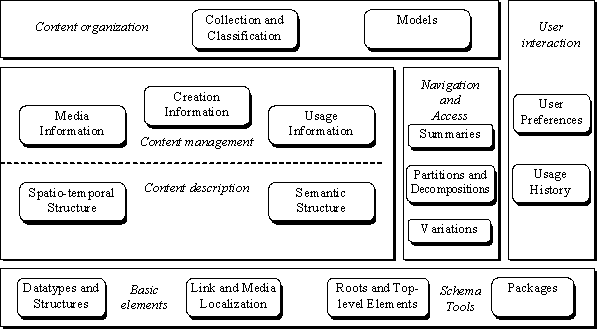
\includegraphics[width=0.8\textwidth]{images/MPEG-7-MDS.png}
\caption{Vue d'ensemble des Schémas de Description (DSs) de la norme MPEG-7}
\label{img:soa:mds}
\end{figure}

Les descriptions produites sont représentées dans un \e{Langage de Description des Définitions} (Description Definition Language, DLL) qui permet de spécifier la syntaxe des Descripteurs, la structure des Schémas de Description ainsi que la sémantique de l'ensemble.
Ce langage permet également de créer ou modifier des Descripteurs, d'étendre ou de modifier les Schémas de Descriptions. 
Le DLL est en réalité XML Schema (\cite{Fallside2004}) agrémenté de quelques types primitifs.

Pour utiliser MPEG-7, il faut également des outils et des directives annexes qui permettent de guider les utilisateurs. 
% définition / implémentation ? 
Dans la partie \e{Systems} de la norme, on trouve ainsi la définition d'outils qui remplissent les fonctions suivantes : codage d'une description MPEG-7 en binaire ; mécanismes de transmissions des descriptions (en binaire ou en texte) à part ou en parallèle du contenu audiovisuel décrit ;  synchronisation entre description et contenu audiovisuel ; gestion des descriptions et de la propriété intellectuelle. 
La partie \e{Reference Software} présente des logiciels de références pour utiliser la norme.
Enfin, la partie \e{Conformance} explicite des directives et des procédures pour s'assurer de la conformité des descriptions produites.

Nous détaillerons dans cette section les Schémas de Description liés à la gestion du contenu (\e{Content Management} dans la Figure \ref{img:soa:mds}) et à la description du contenu (\e{Content Description}).\\


\subsubsection{Gestion du contenu}
MPEG-7 définit trois concepts fondamentaux pour modéliser l'enregistrement d'une réalité en un contenu multimédia et les multiples transformations qu'il est possible de lui appliquer. 
Ainsi, pour chaque modalité d'enregistrement (audio, audiovisuel, photo etc.) MPEG-7 considère la création de trois éléments, une \pc{ContentEntity} (entité de contenu, CE), une \pc{MediaInstance} (instance de média, MI) et un \pc{MediaProfile} (profil de média, MP), voir la Figure \ref{img:soa:media}.
Pour donner une première idée, on peut dire que le fichier créé correspond à la \pc{MediaInstance}, que le \pc{MediaProfile} correspond aux paramétrages de son encodage et que la \pc{ContentEntity} représente le contenu de manière abstraite.

\begin{figure}[ht!]
\centering
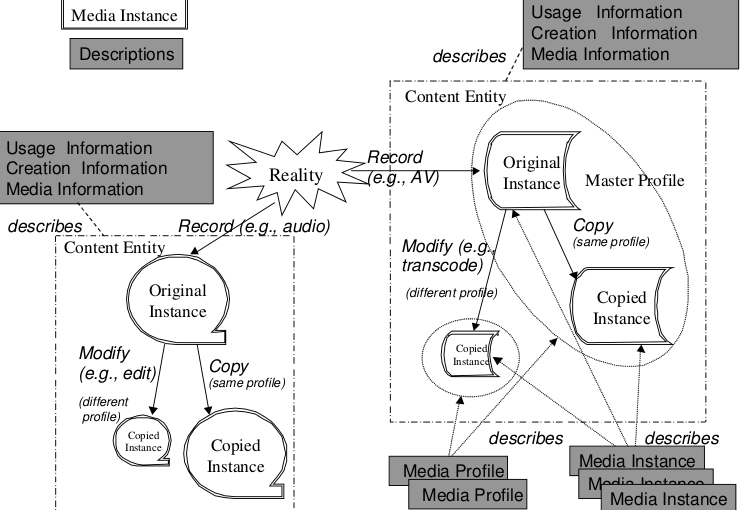
\includegraphics[width=0.8\textwidth]{images/MPEG-7-MediaManagement.png}
\caption{Gestion des contenus dans MPEG-7 à trois niveaux : contenu, instance et profile.}
\label{img:soa:media}
\end{figure}


On remarque qu'il existe cependant des différences entre les \pc{MediaInstance}, entre l'original et ce qui est nommé des \gui{copies} (copied instances). 
Ce qui est particulièrement intéressant pour nous est de constater que la nature de la manipulation entre l'original et les soi-disantes \gui{copies} importe peu (copie technique, réencodage ou montage), car cela crée de toute façon une nouvelle \pc{MediaInstance}. 

À l'inverse, la notion de \pc{MediaProfile} est dépendante de la nature de ces transformations. 
Le \gui{MasterProfile} correspond ainsi aux paramètres d'encodage de la MI d'origine, la première créée. 
Ainsi, dès qu'une différence d'encodage apparaît avec les MI créées ultérieurement, un nouveau \pc{MediaProfile} est créé. 
Il correspond donc à un regroupement de toutes les instances ayant en commun le même encodage. 
%%%% orthographe %%%%
Ce qui paraît troublant néanmoins, est l'amalgame fait entre réencodage et montage. 
Les changements de structure réalisés par le montage semblent en effet bien plus significatif qu'un changement de paramètre d'enregistrement. 
On peut se souvenir de la citation d'\pc{Eisenstein} à ce sujet évoqué en section \ref{sec:prod}.

Enfin, la notion de \pc{ContentEntity} correspond à une entité abstraite permettant de regrouper toutes les versions ultérieures de ce même contenu.
De ce fait, c'est à elle qu'on attache des informations concernant la création, l'usage et le type de média construit. % ??? Sûr ???
Ce regroupement d'informations à ce niveau découle de l'idée que chaque \pc{ContentEntity} définit une forme reconnaissable de contenu, quelque soit les variations apportées.
Encore une fois, l'idée qu'un montage différent n'impacte pas la forme et donc potentiellement l'identité du contenu nous semble ambiguë. 
Il s'agit là d'un de nos points d'achoppement par rapport à la modélisation proposée par la norme. 

\paragraph{Schémas de description}
Détaillons maintenant les trois Schémas de Descriptions proposés par MPEG-7 dans la partie \gui{Content Management}.
Remarquons que ces schémas s'appliquent tous à décrire les \pc{ContentEntity}.
% plus de détails sur les DSs

Le \pc{MediaInformation} est un schéma qui comporte des informations d'identification du CE ainsi qu'un ou plusieurs Profiles d'instances. 
Il faut remarquer que la définition du Profile proposé implique que le moindre changement d'encodage aboutit à la création d'un nouveau Profile en plus de l'instance. 
Il devient alors clair qu'un Profile représente la description d'un groupe d'instances, dont il facilite la gestion.
\begin{liste}
	\item \pc{MediaIdentification} : propose un ou plusieurs identifiants pour le CE.
	\item \pc{MediaProfile} : est composé de plusieurs descripteurs qui détaillent les paramètres et formats utilisés pour encoder une ou plusieurs instances.
	Il s'agit en particulier du \pc{MediaFormat} (pour l'encodage et le format d'encapsulation des données) ; le \pc{MediaInstance} (visant à identifier et localiser les instances) ; le \pc{MediaTranscodingHints} (pour faciliter le réencodage des données) ; le \pc{MediaQuality} (pour détailler la qualité et les défauts). 
\end{liste}


Le \pc{CreationInformation} peut être considéré comme une version étendue à l'audiovisuel des éléments du DCMI. Il comporte les Schémas de Description suivants : 
	\begin{liste}
		\item \pc{Creation} : des métadonnées qui permettent d'identifier le contenu (titre), proposer un résumé et des informations sur les conditions de sa création (créateur et contributeurs avec leur rôle, lieu, date, matériel et paramètrage utilisé).

		\item \pc{Classification} : des éléments de classification du contenu par forme (film, journal télévisé etc.), genre (sport, politique etc.), sujet, langage présent, et des informations sur la diffusion (date, région, public cible, critiques etc.)

		\item \pc{RelatedMaterial} : des métadonnées sur les autres versions d'un même contenu (format, type de média, localisation du média etc.) qui sont ensuite elles-mêmes décrites comme des éléments à part.
	\end{liste}

Le \pc{UsageDescription} est un schéma qui comporte un descripteur détaillant les droits attachés au contenu (\pc{Rights}), un descripteur décrivant les résultats financiers (\pc{FinancialResults}) et des schémas de descriptions sur les détails d'utilisation du contenu (\pc{Availability}) et sur l'historique de son utilisation(\pc{UsageRecord}).
Les droits d'exploitation peuvent en effet porter uniquement sur certains types de distribution (DVD, télédiffusion etc.) ou une certaine période. 
L'historique permet de garder trace des diffusions et de leur audience.


\subsubsection{Description du contenu}
\paragraph{La structure spatio-temporelle du contenu}
MPEG-7 fournit un ensemble de schémas et de descripteurs qui permettent de découper les contenus multimédias de toute les manières possibles. 
Pour cela, la norme définit la notion de \pc{Segment} qui se décline en segment spatial, temporel ou spatio-temporel et sur tout types de média (audio, image, audiovisuel, multimédia). 
Chaque segment peut se décomposer en d'autres segments suivant la structure d'un arbre. 
De plus, ces segments peuvent être connectés entre eux ou pas, c'est-à-dire spécifier trois zones connexes ou pas d'une image ou bien trois séquences temporelles qui se suivent ou pas. 
Les Segments peuvent également n'être valable que pour une source média particulière, comme une piste audio comportant la musique.

Un point particulièrement important est que chacun de ces \pc{Segment} est considéré comme une \pc{ContentEntity}. 
On peut donc utiliser les schémas de \pc{MediaInformation}, \pc{CreationInformation} et de \pc{UsageDescription} pour les décrire ainsi qu'un schéma \pc{Semantic} que nous décrivons ci-après. 
En plus de cela, de nombreux schémas spécifiques à la nature du média existent pour décrire le signal de manière analytique. 


\paragraph{Aspects sémantiques}
Le schéma \pc{Semantic} permet de décrire le monde qui est présenté aux lecteurs dans le contenu audiovisuel. 
Il s'agit d'une description basée sur les évènements (\pc{Event}) ayant lieu à tel moment (\pc{SemanticTime}), à tel endroit (\pc{SemanticPlace}), et auxquels participent des objets (\pc{Object}) ou des agents (\pc{AgentObject}). 
La description peut être raffinée en utilisant des concepts (\pc{Concept}), en détaillant les attributs d'une entité (\pc{SemanticState}) ou bien les relations entre entités (\pc{SemanticRelation}).
À noter, que ces relations peuvent tout autant porté sur les évènements se déroulant dans le contenu (par exemple, l'agent A est bénéficiaire d'un évènement B) ou bien entre un contenu et des entités sémantiques (par exemple, l'image A est une référence à l'objet B).

% \begin{liste}
% 	\item SemanticDescription
% 	\item ModelDescription
% 	\item SummaryDescription
% 	\item ViewDescription
% 	\item VariationDescription
% \end{liste}




%To address the standard's inherent annotation ambiguity and bring it to a Semantic Web level, \cite{Arndt2007} performed a selected formalization based on the DOLCE foundational ontology. In a sense, they have provided us with a knowledge representation version of MPEG-7.\\



% Ontologies basées sur MPEG-7 : \cite{Dasiopoulou2009}
%=============
\subsection{Core Ontology for MultiMedia}
% \addcontentsline{toc}{subsubsection}{Core Ontology for MultiMedia}
\cite{Arndt2009} ; \cite{Arndt2007} ; \cite{Staab2008} 
MPEG-7 has been widely used to represent low-level features and to associate them with parts of multimedia material \cite{VanOssenbruggen2004}. \cite{Nack2005a} and \cite{Arndt2009} pointed two major drawbacks to the use of MPEG-7 in a Semantic Web environment: 1) its representation as a XML Schema do not provide direct integration with other knowledge representation standards 2) the inherent syntactic and semantic ambiguity of content annotation descriptors. 

Several works have tried to formalize the standards partially, \cite{Hunter2001} and \cite{Tsinaraki2004}. \cite{Garcia2005} created automatically a full OWL conversion. However, these works have never provided a clear solution to the syntactic and semantic ambiguity of MPEG-7 content description. The Core Ontology for MultiMedia (COMM) proposes to redesign MPEG-7 with respects to the Semantic Web and knowledge representation standards \cite{Arndt2007}. Using the DOLCE foundational ontology as a modeling basis, they performed a selected formalization of MPEG-7 descriptor and thus clarified modeling patterns. 




%=============
\subsection{MPEG-21}
% \addcontentsline{toc}{subsubsection}{MPEG-21}
% \cite{Burnett2003} ; \cite{Garcia2010} ? 
%Creation Value Chain
Along with MPEG-7, the MPEG-21 Multimedia Framework \cite{Burnett2003} offers a valuable perspective on future practices in content management, distribution and consumption. The recent interest in content value chains modeling presented in \cite{Garcia2010} shows some similarities with our audiovisual object modeling approach. There is still an open debate about the modeling of the various forms or facets that content can take during its production. Many approaches rely on, adapt or extend the original FRBR Group 1 concepts of \e{Work}, \e{Expression}, \e{Manifestation} and \e{Item}. 
For instance, the Media Value Chain Ontology (MVCO) \cite{Rodriguez-Doncel2009}, \cite{Rodriguez-Doncel2010} is included as the Part 19 of the MPEG-21 standard. 
The authors merge the concepts of Expression and Manifestation. Moreover, they also propose a new concept of Product for asset which needs to be licensed before publishing. 
% Citer également : Jane Hunter -- Reconciling MPEG-7 and MPEG-21 Semantics through a Common Event-Aware Metadata Model




%=============
\subsection{TV Anytime}
% \addcontentsline{toc}{subsubsection}{TV Anytime}
\cite{Evain2000} ; \cite{Tsinaraki2004} ; \cite{Tsinaraki2005}

%=============
\subsection{Material eXchange Format : Description Metadata Scheme-1}
% \addcontentsline{toc}{subsubsection}{Material eXchange Format : Description Metadata Scheme-1}
\cite{Marcos2009}

%=============
\subsection{OntoMedia : la convergence des modèles}
\cite{Lee2012}, \cite{Burger2011}



%=============================
%=============================
\subsection{Descriptions métiers}
Script, Storyboard (\cite{Martin2005}, \cite{ThiBui2003}) etc.
Réappropriations dans le champ informatique : \cite{Chakravarthy2009b} ; \cite{Chakravarthy2009c}

Another trail of research has emerged recently. In comparison to the previous approach, it does not attack the multimedia description from below (with signal processing techniques) but from above. The principles is to represent the knowledge included in documents related to the multimedia content. It can be a web-page where the image is published and commented by others \cite{Simperl2009} or more specific documents related to the production context. \cite{Chakravarthy2009b} and \cite{Chakravarthy2009c} take interest in the knowledge of film direction. They propose a semantic model which captures the information typically included in a storyboard or screenplay. They also provide a system to capture the director's demands and assist her/him during the shooting. 
A similar work has been carried out by \cite{VanRijsselbergen2009} but with distinct goal and language. Their MovieScriptMarkupLanguage (MSML) captures the information of a shooting script with a particular attention to the details of set equipment's and actor's positions. The related Scoop system \cite{Cardinaels2008} provides its user 3D model of the set as well as the shots taken by the camera in a given position and settings. The overall objective is to provide an shooting-set 3D simulation to assist the production team in their preparation.\\






%=============================
%=============================
\subsection{Systèmes informatiques}
\cite{Tsinaraki2005} ; \cite{Tsinaraki2004} ; \cite{Dasiopoulou2009} (dans Gestion ?)



% Our approach follows this trend of research with different focus and objectives than the works presented. We consider the shooting script as the main production document to describe the video shots. The focus is on the realization of these shots, not the preparation or direction of the production. It does not assist the same people and do not provide exactly the same pieces of information. As we demonstrated above, a Semantic Script can assist the cameraman at shooting time and the professional editor when reviewing. 
% In comparison to the COMM ontology, our model offers an additional representation layer with describe the editorial structure of audiovisual objects (Opus, MediaAsset, EditorialObject). With the Semantic Script, we provide a way to predefine a structure and capture intentions that are inherent to the audiovisual production process. COMM represents a MPEG-7 flavored description of video files and also the way this description has been produced by human or algorithms. This indexing is made after the video production and do not provide any mean to retain information from the context of production.

